\documentclass[12pt]{article}
\usepackage{amsmath}
\usepackage{amssymb}
\usepackage{amsthm}
\usepackage[left=2cm, right=2cm, top=2cm]{geometry}
\usepackage{enumitem}
\usepackage{graphicx}
\usepackage{color}   %May be necessary if you want to color links
\usepackage{hyperref}
\hypersetup{
    colorlinks=true, %set true if you want colored links
    linktoc=all,     %set to all if you want both sections and subsections linked
    linkcolor=blue,  %choose some color if you want links to stand out
}
\usepackage{bbm}
\usepackage{soul}
\usepackage{tcolorbox}
\usepackage{tikz}
\usepackage{graphicx}
\usepackage{draftwatermark}
\SetWatermarkText{
\includegraphics[scale=5]{JoeWest.png}}
\tcbuselibrary{theorems}
\tcbuselibrary{breakable}

\newtcbtheorem[number within=section]{mythm}{Theorem}%
{colback=green!5,colframe=green!35!black,fonttitle=\bfseries,unbreakable}{th}
\newtcbtheorem[use counter from=mythm]{mydef}{Definition}%
{colback=blue!5,colframe=blue!35!black,fonttitle=\bfseries,unbreakable}{de}
\newtcbtheorem[use counter from=mythm]{myrem}{Remark}%
{colback=white!5,colframe=white!35!black,fonttitle=\bfseries,unbreakable}{re}
\newtcbtheorem[use counter from=mythm]{myex}{Example}%
{colback=orange!5,colframe=orange!35!black,fonttitle=\bfseries,unbreakable}{ex}
\newtcbtheorem[use counter from=mythm]{myprop}{Proposition}%
{colback=green!5,colframe=green!35!black,fonttitle=\bfseries,unbreakable}{pr}
\newtcbtheorem[use counter from=mythm]{mylem}{Lemma}%
{colback=green!5,colframe=green!35!black,fonttitle=\bfseries,unbreakable}{le}
\newtcbtheorem[use counter from=mythm]{mycor}{Corollary}%
{colback=green!5,colframe=green!35!black,fonttitle=\bfseries,unbreakable}{co}

\newcommand{\R}{\mathbb{R}}
\newcommand{\N}{\mathbb{N}}
\newcommand{\Z}{\mathbb{Z}}
\newcommand{\Q}{\mathbb{Q}}
\newcommand{\Log}{\text{Log}}
\renewcommand{\C}{\mathbb{C}}
\newcommand{\inv}{^{-1}}

\setcounter{tocdepth}{3}
\setlength\parindent{0pt}
\hyphenpenalty 10000

\title{PMATH 332}
\author{Max Zhu}

\begin{document}
	\maketitle
	\section{2019-06-14}	
	\begin{myex}{Most important example in this course}{}
		Evaluate $\int_C\frac{1}{z}dz$ where $C$ is the unit circle, traversed once counter-clockwise.\\
		
		The anti-derivative of $\frac{1}{z}$ is $\log(z)$, but this has a branch cut on $C$ so we can't use it directly.\\
		
		Method 1: Parametrize $C$ as $z(t)=e^{it}$ for $t\in[0, 2\pi]$. Then,
		\begin{align*}
			\int_C\frac{1}{z}dz&=\int_{0}^{2\pi}\frac{1}{e^{it}}\cdot ie^{it}dt\\
			&=2\pi i
		\end{align*}
		
		Method 2: Separate the circle into two semicircles, $C_1$ and $C_2$. Define $C_1$ to go from $-i$ to $i$ and $C_2$ to go from $i$ to $-i$. Then,
		\begin{align*}
			\int_{C_1}\frac{1}{z}dz&=[\Log(z)]_{-i}^{i}\\
			&=\Log(i)-\Log(-i)\\
			&=i\frac{\pi}{2}-i\frac{-\pi}{2}\\
			&=i\pi
		\end{align*}
		For $C_2$, use $\Log_0(z)$ instead to avoid the branch cut.
		\begin{align*}
			\int_{C_2}\frac{1}{z}dz&=[\Log_0(z)]_{i}^{-i}\\
			&=\Log_0(-i)-\Log_0(i)\\
			&=i\frac{3\pi}{2}-i\frac{\pi}{2}\\
			&=i\pi
		\end{align*}
		So,
		\begin{align*}
			\int_C\frac{1}{z}dz&=\int_{C_1}\frac{1}{z}dz+\int_{C_2}\frac{1}{z}dz\\
			&=2\pi i
		\end{align*}
	\end{myex}
	
	\begin{myrem}{}{}
		\begin{itemize}
			\item For any circle of radius $R$, you will still get $2\pi i$.
			\item If you traverse the circle twice, you will get $4\pi i$.
			\item If you traverse backwards, you will get $-2\pi i$.
		\end{itemize}
	\end{myrem}
	
	\begin{mydef}{Continuously deformable}{}
		A closed contour $C$ is said to be \underline{continuously deformable} to a contour $C_1$ in a domain $D$ if there exists a function $z(s, t)$ which is continuous on $s, t\in[0, 1]$ such that:
		\begin{itemize}
			\item $z(s, t)$ is a closed contour in $D$ for all $s\in[0, 1]$.
			\item $z(0, t)$ parametrizes $C$.
			\item $z(1, t)$ parametrizes $C_1$.
		\end{itemize}
	\end{mydef}
	
	\begin{myex}{}{}
		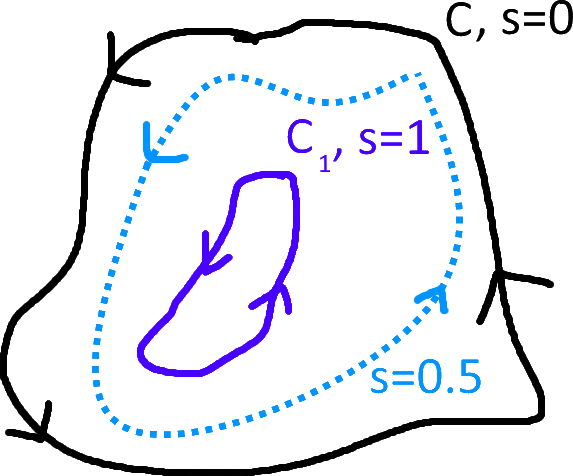
\includegraphics[scale=1]{Notes1.png}
	\end{myex}
	
	\begin{mythm}{Deformation invariance theorem}{}
		Let $f$ be analytic in domain $D$ containing contours $C_1$ and $C_2$. If $C_1$ can be continuously deformed into $C_2$, then
		\begin{align*}
			\oint_{C_1}f(z)dz&=\oint_{C_2}f(z)dz
		\end{align*}
		\begin{proof}
			Too long to fit in these notes.
		\end{proof}
	\end{mythm}
	
	\begin{mydef}{Simply connected domain}{}
		A domain $D$ is \underline{simply connected} if every ``loop" in $D$ can be continuously deformed into a point while remaining in $D$.
		
		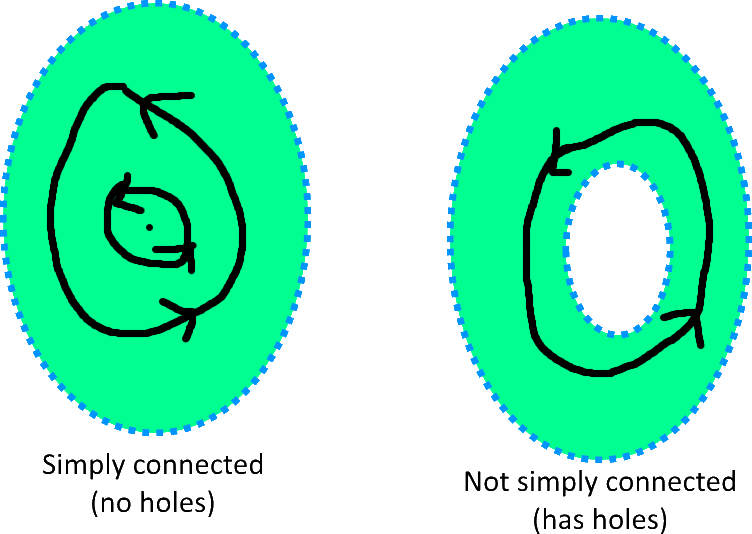
\includegraphics[scale=0.7]{Notes2.png}
	\end{mydef}
	
	\begin{mythm}{Cauchy's integral theorem (aka Cauchy-Coursat theorem)}{}
		If $f$ is analytic in a simply connected domain $D$, and $C$ is a closed contour in $D$, then
		\begin{align*}
			\oint_Cf(z)dz&=0
		\end{align*}
		\begin{proof}
			Since $D$ is simply connected, $C$ can be continuously deformed into a point, so the result holds by deformation invariance theorem.
		\end{proof}
	\end{mythm}
	
	\begin{mycor}{}{}
		If $f$ is analytic then $f$ is infinitely anti-differentiable.
		\begin{proof}
			By Cauchy's integral theorem, $\oint_Cf(z)dz=0$ for any closed contour $C$, and so by theorem $f$ is anti-differentiable. The anti-derivative of $f$ must be analytic, so the anti-derivative itself must also be anti-differentiable, etc.
		\end{proof}
	\end{mycor}
	
	\begin{myex}{}{}
		We have
		\begin{align*}
			\oint_C\frac{1}{z}dz&=2\pi i
		\end{align*}
		for any positively oriented contour $C$ enclosing the origin. We could shift this:
		\begin{align*}
			\oint_C\frac{1}{z-z_0}dz&=\begin{cases}
				2\pi i&\;\text{if }z_0\text{ is inside }C\\
				0&\;\text{otherwise}
			\end{cases}
		\end{align*}
	\end{myex}
\end{document}